\chapter{Desenvolvimento reprodutivo e controle da floração}\label{ch:b2:plant-flowering}

Um produtor de crisântemos consegue fazer uma estufa florescer no Natal
ou na Páscoa ligando e desligando as luzes; um trigo de inverno semeado
na primavera nunca floresce, porque não passou frio; um carrapicho que
passou por uma única noite mais longa que seu comprimento crítico está
comprometido com a floração, aconteça o que acontecer depois. Uma
planta não tem calendário, mas tem relógios, termômetros e medidores de
luz, e decide uma vez por ano, com base neles, converter um \omterm{def:b2:plant-meristems:meristem}{meristema}
que vinha produzindo folhas num \omterm{def:b2:plant-meristems:meristem}{meristema} que produzirá uma \omterm{def:b2:angiosperm-reproduction:flower}{flor}. Este
capítulo acompanha essa decisão, da folha que mede a noite ao
\omterm{def:b2:plant-meristems:meristem}{meristema} que muda de programa, depois a construção da \omterm{def:b2:angiosperm-reproduction:flower}{flor} por um
código de genes, e a transição inversa na outra ponta do ciclo: a
\omterm{def:b2:angiosperm-reproduction:seed}{semente} que não germina até receber a informação de que a estação é
propícia.

\section{A transição para a floração}

\begin{definition}[Transição e indução florais]\label{def:b2:plant-flowering:transition}
\index{transição floral}\index{indução floral}\index{meristema de inflorescência}
Um \omterm{def:b2:plant-meristems:meristem}{meristema apical caulinar} vegetativo produz folhas com uma gema em
cada axila, indefinidamente. Na \emph{transição floral}, ele se torna um
\emph{\omterm{def:b2:plant-meristems:meristem}{meristema} de inflorescência}, que produz brácteas e, nas axilas
delas, \emph{\omterm{def:b2:plant-meristems:meristem}{meristemas} florais}, cada um dos quais é determinado:
produz sépalas, pétalas, \omterm{def:b2:angiosperm-reproduction:flower}{estames} e \omterm{def:b2:angiosperm-reproduction:flower}{carpelos} e depois para. A mudança é
desencadeada pela \emph{indução floral} --- um sinal, vindo das folhas
ou surgido da própria fisiologia da planta, que ativa os genes de
identidade do \omterm{def:b2:plant-meristems:meristem}{meristema}. As plantas anuais florescem uma vez e morrem;
as perenes florescem todos os anos a partir de alguns \omterm{def:b2:plant-meristems:meristem}{meristemas} e
mantêm outros vegetativos. O momento decide se o \omterm{def:b2:plant-life-cycles:heterospory}{pólen} encontra o
\omterm{def:b2:angiosperm-reproduction:flower}{estigma}, se as \omterm{def:b2:angiosperm-reproduction:seed}{sementes} amadurecem antes da geada e se a \omterm{def:b2:angiosperm-reproduction:flower}{flor} se abre
quando seu polinizador está voando: ele está sob forte seleção, e as
plantas desenvolveram várias maneiras de ler a estação.
\end{definition}

\begin{proposition}[Fotoperiodismo: a planta mede a noite]\label{prop:b2:plant-flowering:photoperiod}
\index{fotoperiodismo}\index{planta de dia curto}\index{planta de dia longo}\index{fitocromo}
Muitas plantas florescem em resposta ao comprimento do dia. As
\emph{\omterm{prop:b2:plant-flowering:photoperiod}{plantas de dia curto}} (crisântemo, soja, arroz, carrapicho)
florescem quando o dia é mais curto que um comprimento crítico --- no
outono ou na primavera; as \emph{\omterm{prop:b2:plant-flowering:photoperiod}{plantas de dia longo}} (espinafre,
trigo, trevo, \emph{Arabidopsis}), quando ele é mais longo --- no início
do verão; as plantas \emph{neutras} (tomate, milho) florescem quando
atingem tamanho suficiente. O que a planta mede é, na verdade, o
comprimento da \emph{noite} ininterrupta: uma \omterm{prop:b2:plant-flowering:photoperiod}{planta de dia curto} é uma
planta de noite longa, e um lampejo de luz no meio de uma noite longa
cancela seu efeito, ao passo que um período de escuro num dia longo
não o faz. A medida é feita nas \emph{folhas}, pelo pigmento
\emph{fitocromo} --- uma proteína que alterna entre uma forma que
absorve o vermelho e uma forma que absorve o vermelho extremo a cada
fóton que capta, de modo que seu estado registra a luz ---, lido em
relação a um \emph{relógio circadiano} interno de cerca de vinte e
quatro horas: a floração é desencadeada quando a luz coincide com uma
fase particular do relógio, o que só acontece no comprimento de dia
certo.
\end{proposition}
\begin{proof}[Evidências]
Garner e Allard (1920) verificaram que um tabaco mutante só florescia
nos dias curtos de uma estufa de inverno, e que sojas semeadas a
intervalos ao longo do verão floresciam todas juntas em setembro: o
comprimento do dia, e não a idade ou a temperatura, fixava a data.
Hamner e Bonner (1938) mostraram com o carrapicho que uma única noite
longa bastava, que um minuto de luz no meio da noite abolia o efeito e
que encurtar o dia sem mudar a noite não induzia. Borthwick e Hendricks
(1952) verificaram que a luz mais eficaz era a vermelha e que a luz
vermelha extrema dada logo depois da vermelha a cancelava --- a
assinatura do fitocromo, isolado em 1959. Enxertar uma única folha
induzida numa planta não induzida fazia a planta inteira florescer: a
folha exporta um sinal.
\end{proof}

\begin{omfigure}
\begin{tikzpicture}[every node/.style={font=\scriptsize}]
  \foreach \y/\lab/\res in {3.6/{dia longo, noite curta}/{sem flor}, 2.7/{dia curto, noite longa}/{floresce}, 1.8/{noite longa cortada por um lampejo}/{sem flor}, 0.9/{dia longo interrompido por escuro}/{sem flor}} {
    \node[anchor=east, align=right] at (-0.2,\y) {\lab};
    \node[anchor=west, omThm] at (8.6,\y) {\res};
  }
  % bars: 24 h = 8 cm; light yellow, dark grey
  \fill[omExo!30] (0,3.4) rectangle (8,3.8); \fill[yellow!50!orange!40] (0,3.4) rectangle (5.4,3.8);
  \fill[omExo!30] (0,2.5) rectangle (8,2.9); \fill[yellow!50!orange!40] (0,2.5) rectangle (3.0,2.9);
  \fill[omExo!30] (0,1.6) rectangle (8,2.0); \fill[yellow!50!orange!40] (0,1.6) rectangle (3.0,2.0); \fill[yellow!50!orange!40] (5.4,1.6) rectangle (5.55,2.0);
  \fill[omExo!30] (0,0.7) rectangle (8,1.1); \fill[yellow!50!orange!40] (0,0.7) rectangle (5.4,1.1); \fill[omExo!30] (2.6,0.7) rectangle (2.9,1.1);
  \draw[thick, ->] (0,0.3) -- (8.2,0.3); \foreach \x/\l in {0/0,2/6,4/12,6/18,8/24} \draw (\x,0.35) -- (\x,0.25) node[below] {\l};
  \node[below] at (4,-0.05) {horas};
  \draw[dashed, omDef] (5.4,0.3) -- (5.4,4.0); \node[omDef, above] at (5.4,4.0) {comprimento crítico da noite};
\end{tikzpicture}

{\small O carrapicho de Hamner e Bonner, uma \omterm{prop:b2:plant-flowering:photoperiod}{planta de dia curto}. Ele
floresce após uma noite mais longa que o comprimento crítico; um minuto
de luz no meio da noite cancela a indução, ao passo que um período de
escuro durante o dia não. A planta mede a noite.}
\end{omfigure}

\begin{definition}[Florígeno]\label{def:b2:plant-flowering:florigen}
\index{florígeno}\index{FLOWERING LOCUS T}
O sinal que a folha exporta foi chamado de \emph{florígeno} em 1937 e
identificado setenta anos depois como uma pequena proteína, o produto
do gene \emph{FLOWERING LOCUS T} (FT). Na folha, o relógio e o
fitocromo juntos só ativam o FT quando o comprimento do dia é o certo
(em \emph{Arabidopsis}, uma \omterm{prop:b2:plant-flowering:photoperiod}{planta de dia longo}, quando a luz coincide
com o pico vespertino do ativador CONSTANS, controlado pelo relógio);
a proteína FT entra no floema, viaja com o fluxo de açúcar até o ápice
caulinar e ali, com uma proteína parceira, ativa os genes que convertem
o \omterm{def:b2:plant-meristems:meristem}{meristema}. A mesma proteína é o florígeno do arroz, uma \omterm{prop:b2:plant-flowering:photoperiod}{planta de dia
curto}, na qual o relógio a conecta de modo inverso. Os experimentos de
enxertia, o transporte da proteína no floema e a floração de plantas
em que o FT é expresso a partir de um promotor específico da folha
concordam todos: a \omterm{def:b2:angiosperm-reproduction:flower}{flor} é decidida na folha e executada na gema.
\end{definition}

\begin{omfigure}
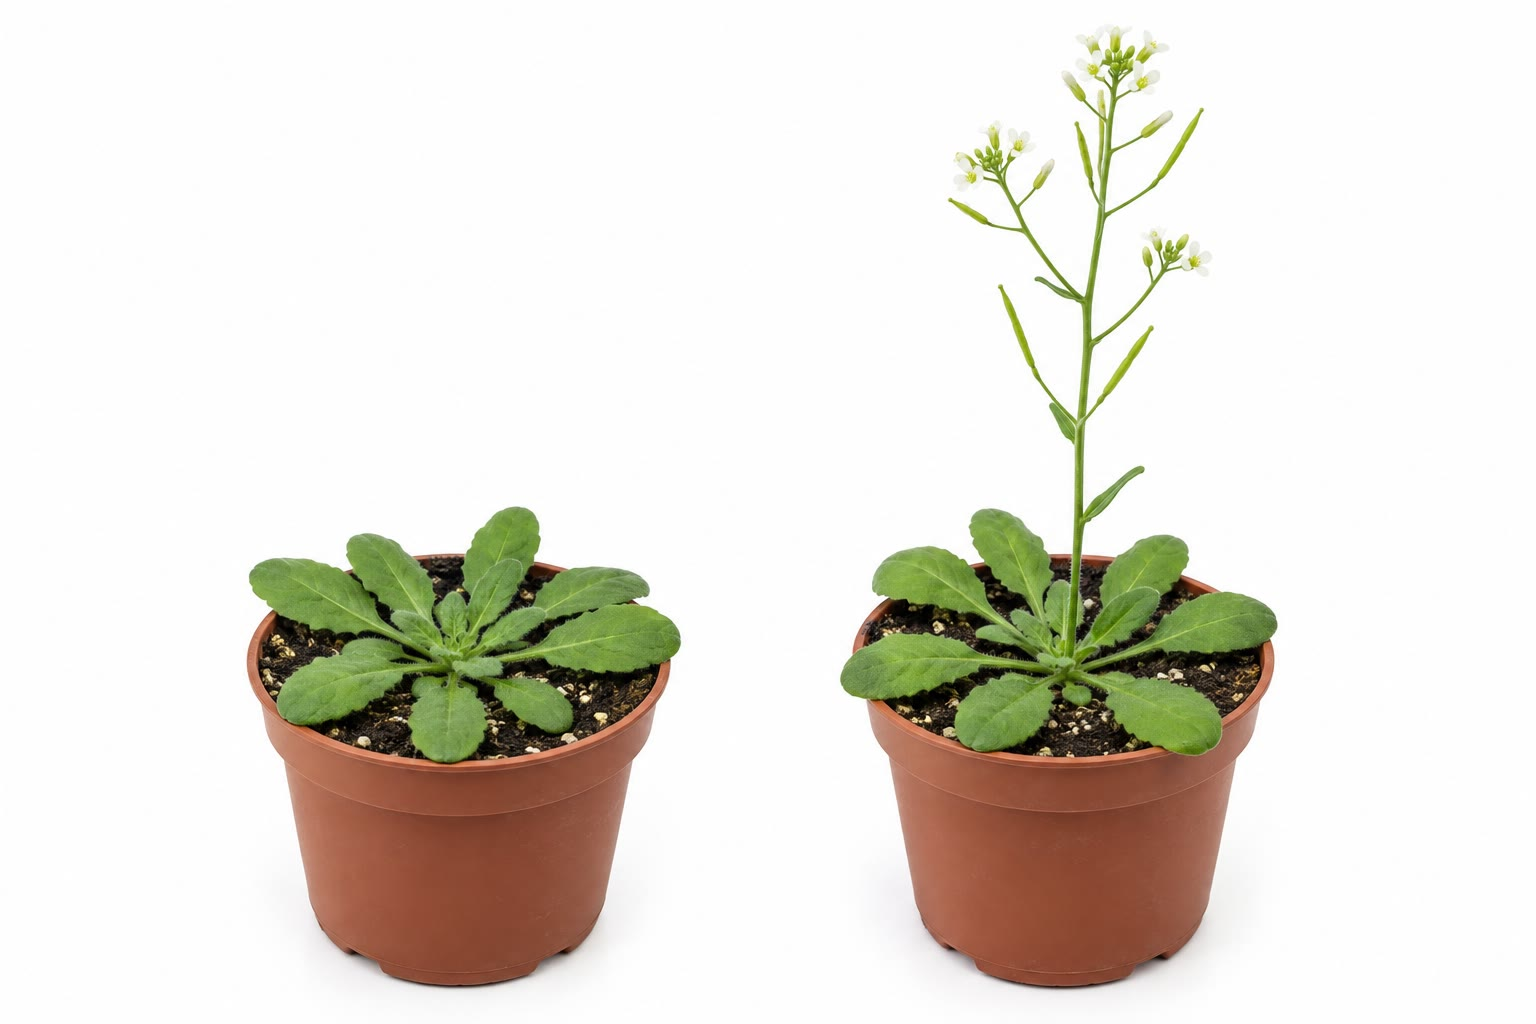
\includegraphics[width=0.58\linewidth]{images/book4/ai/b4-14-arabidopsis-daylength.jpg}

{\small \emph{Arabidopsis}, uma \omterm{prop:b2:plant-flowering:photoperiod}{planta de dia longo}: em dias curtos,
uma roseta de folhas; transferida para dias longos, ela espiga e
floresce em poucas semanas.}
\end{omfigure}

\begin{proposition}[Vernalização: a planta conta o frio]\label{prop:b2:plant-flowering:vernalisation}
\index{vernalização}\index{FLOWERING LOCUS C}
Os cereais de inverno, as bienais (cenoura, repolho, dedaleira) e muitas
perenes de climas frios não florescem antes de passar semanas de frio
--- a \emph{vernalização} ---, o que garante que uma planta que germina
no outono espere a primavera, em vez de florescer em plena geada. O
frio é percebido pelo próprio \omterm{def:b2:plant-meristems:meristem}{meristema}, e não pelas folhas; ele não
pode ser substituído por nenhum outro tratamento; e seu efeito é
lembrado durante o resto do crescimento da planta, ao longo de
centenas de divisões celulares, mas não através da \omterm{def:b2:meiosis-heredity:meiosis}{meiose} --- toda
\omterm{def:b2:angiosperm-reproduction:seed}{semente} começa não vernalizada. Em \emph{Arabidopsis}, a memória é um
gene, o \emph{\omterm{prop:b2:plant-flowering:vernalisation}{FLOWERING LOCUS C}} (FLC), cujo produto reprime a
floração: semanas de frio o silenciam progressivamente, cobrindo sua
cromatina com marcas repressivas; o silenciamento é copiado a cada
divisão e apagado no embrião. A planta \emph{integra}, assim, o frio ao
longo do tempo --- alguns dias frios não contam ---, e um mutante sem
FLC não precisa de inverno.
\end{proposition}

\begin{theorem}[Por que a integração protege contra uma falsa primavera]\label{thm:b2:plant-flowering:integration}
Suponha que um repressor seja silenciado a uma taxa constante $\alpha$
por dia de frio, de modo que, após $n$ dias frios, a fração ainda ativa
seja $f_n = e^{-\alpha n}$, e que a floração seja permitida quando
$f < f_c$. O número de dias frios necessários é
$n_c = \ln(1/f_c)/\alpha$, e --- como o silenciamento é estável --- os
dias frios não precisam ser consecutivos: o que conta é o total. Uma
planta com $n_c = 40$ dias não é enganada por uma quinzena de degelo em
janeiro nem por uma onda de frio em outubro; uma planta que só
percebesse a temperatura do momento floresceria na primeira semana
quente. A mesma integração, com um limiar, é o modo como a planta lê o
comprimento do dia acumulado antes de se comprometer; ambas são
exemplos de um sistema que responde à \emph{integral} de um sinal, e
não a seu valor instantâneo.
\end{theorem}
\begin{proof}
Se cada dia frio silencia uma fração $\alpha$ das cópias ativas
restantes (ou da cromatina ainda não marcada), a fração ativa obedece a
$f_{n+1} = (1 - \alpha)f_n \approx e^{-\alpha}f_n$, donde
$f_n = e^{-\alpha n}$, sendo $n$ o número de dias frios; a desigualdade
$e^{-\alpha n} < f_c$ dá $n > \ln(1/f_c)/\alpha$. Os dias que não são
frios nem acrescentam nem subtraem, pois as marcas são estáveis, de
modo que só o total importa.
\end{proof}

\section{A construção da flor: o modelo ABC}

\begin{proposition}[O modelo ABC]\label{prop:b2:plant-flowering:abc}
\index{modelo ABC}\index{gene homeótico!floral}
Um \omterm{def:b2:plant-meristems:meristem}{meristema} floral forma quatro verticilos concêntricos: sépalas,
pétalas, \omterm{def:b2:angiosperm-reproduction:flower}{estames}, \omterm{def:b2:angiosperm-reproduction:flower}{carpelos}. Suas identidades são fixadas por três
classes de \emph{genes homeóticos}, que agem em anéis sobrepostos: a
classe A sozinha, no verticilo 1, dá sépalas; A e B juntas, no
verticilo 2, dão pétalas; B e C juntas, no verticilo 3, dão \omterm{def:b2:angiosperm-reproduction:flower}{estames}; C
sozinha, no verticilo 4, dá \omterm{def:b2:angiosperm-reproduction:flower}{carpelos}. A e C se reprimem mutuamente, de
modo que, onde uma se perde, a outra se espalha pela \omterm{def:b2:angiosperm-reproduction:flower}{flor} inteira. As
regras preveem todos os mutantes simples: sem B, a \omterm{def:b2:angiosperm-reproduction:flower}{flor} é
sépala--sépala--carpelo--carpelo; sem C, é
sépala--pétala--pétala--sépala, com outra \omterm{def:b2:angiosperm-reproduction:flower}{flor} dentro, pois C também
detém o \omterm{def:b2:plant-meristems:meristem}{meristema}; sem A, é carpelo--estame--estame--carpelo. A maioria
desses genes codifica \omterm{prop:b2:cell-differentiation:transcriptional}{fatores de transcrição} de uma mesma família
(MADS-box), e uma quarta classe, E, é necessária para as três funções;
expressar B e C juntas numa folha a transforma num órgão semelhante a
um \omterm{def:b2:angiosperm-reproduction:flower}{estame}. As \omterm{def:b2:angiosperm-reproduction:flower}{flores} dobradas dos jardins --- rosas, peônias, camélias
--- são mutantes da classe C, com os \omterm{def:b2:angiosperm-reproduction:flower}{estames} transformados em pétalas
extras.
\end{proposition}
\begin{proof}[Evidências]
Coen e Meyerowitz (1991) compararam os mutantes homeóticos de
\emph{Arabidopsis} e da boca-de-leão: em ambas, três classes de \omterm{def:b2:genome-diversification:mutation}{mutação}
transformavam cada uma dois verticilos adjacentes, nos mesmos pares, e
as combinações de mutantes se comportavam como o modelo prevê (o
triplo mutante só forma folhas). A clonagem mostrou que os genes são
\omterm{prop:b2:cell-differentiation:transcriptional}{fatores de transcrição} expressos nos anéis previstos; colocar um gene B
sob um promotor ativo nos quatro verticilos dava
pétala--pétala--estame--estame.
\end{proof}

\begin{omfigure}
\begin{tikzpicture}[every node/.style={font=\scriptsize}]
  % four whorls as columns
  \foreach \x/\w in {0/{verticilo 1}, 2.2/{verticilo 2}, 4.4/{verticilo 3}, 6.6/{verticilo 4}} \node[above] at (\x+0.9,3.3) {\w};
  \fill[omDef!35] (0,2.4) rectangle (4.2,3.1); \node at (2.1,2.75) {A};
  \fill[omProp!40] (2.2,1.6) rectangle (6.4,2.3); \node at (4.3,1.95) {B};
  \fill[omThm!30] (4.4,0.8) rectangle (8.6,1.5); \node at (6.5,1.15) {C};
  \foreach \x/\o in {0/sépalas, 2.2/pétalas, 4.4/estames, 6.6/carpelos} \node[below, align=center] at (\x+0.9,0.6) {\o};
  \node[anchor=west, align=left] at (9.2,3.0) {tipo selvagem: A, AB, BC, C};
  \node[anchor=west, align=left] at (9.2,2.3) {sem B: sépala, sépala, carpelo, carpelo};
  \node[anchor=west, align=left] at (9.2,1.6) {sem C: sépala, pétala, pétala, sépala\ldots};
  \node[anchor=west, align=left] at (9.2,0.9) {sem A: carpelo, estame, estame, carpelo};
\end{tikzpicture}

{\small O \omterm{prop:b2:plant-flowering:abc}{modelo ABC}. Três classes de genes em anéis sobrepostos fixam as
quatro identidades de órgão; perder uma classe converte dois verticilos,
e as \omterm{def:b2:angiosperm-reproduction:flower}{flores} mutantes são exatamente as previstas.}
\end{omfigure}

\begin{omfigure}
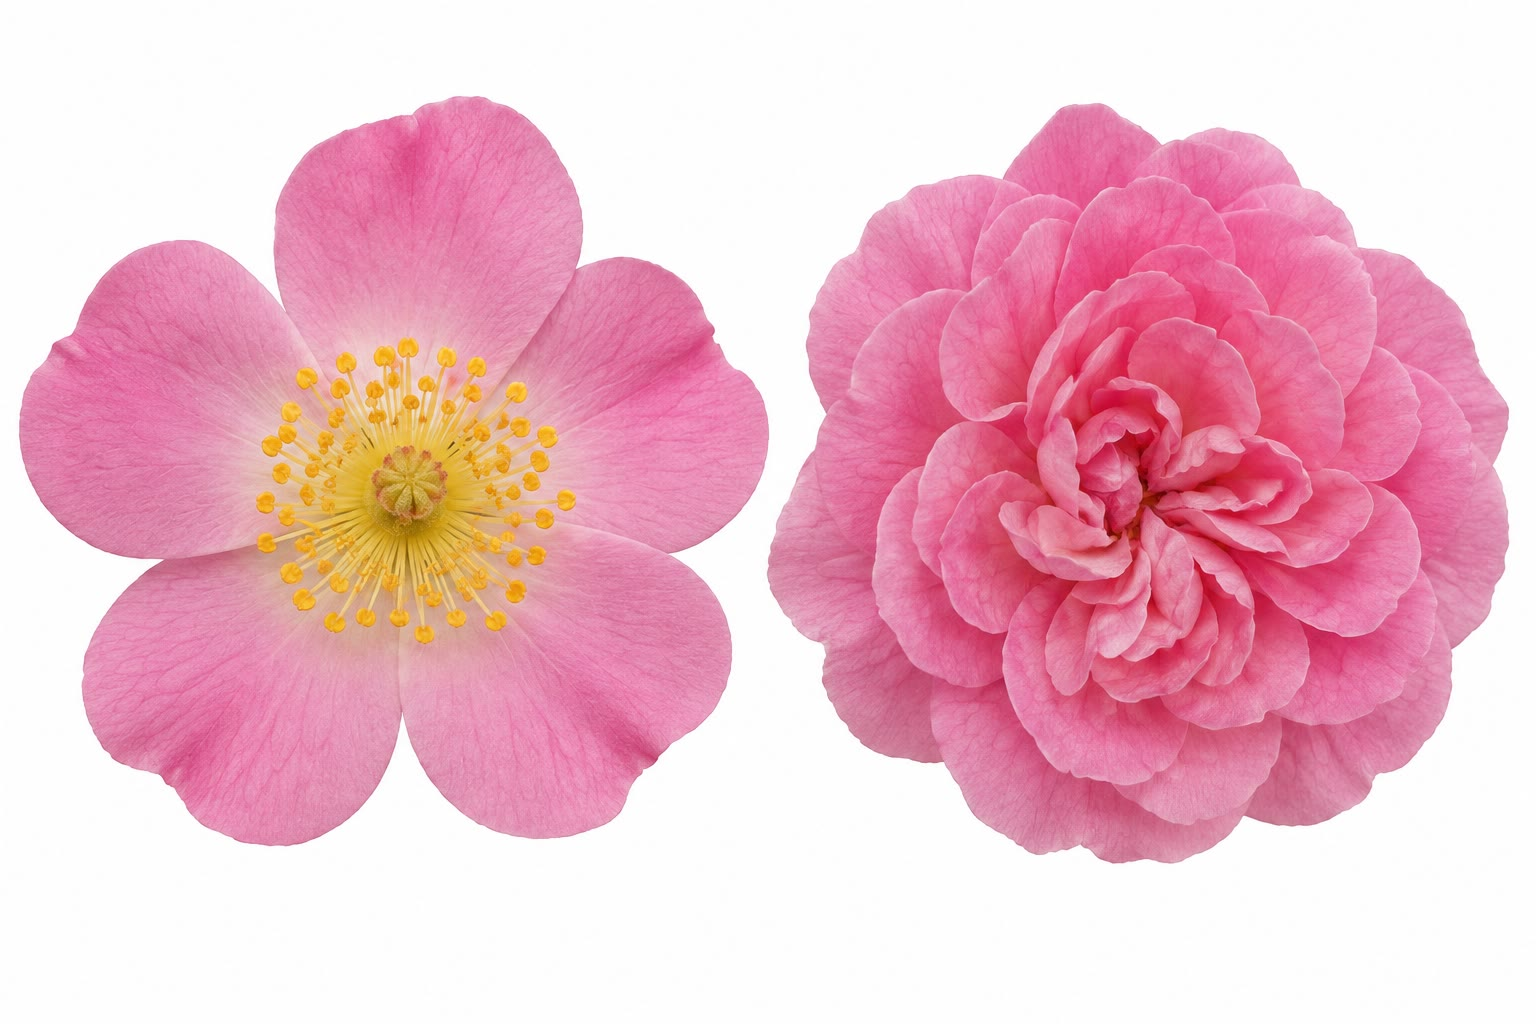
\includegraphics[width=0.58\linewidth]{images/book4/ai/b4-14-double-flower.jpg}

{\small Uma \omterm{def:b2:angiosperm-reproduction:flower}{flor} selvagem ao lado de uma forma dobrada: os \omterm{def:b2:angiosperm-reproduction:flower}{estames} se
tornaram pétalas --- um mutante da classe C, selecionado pelos
jardineiros durante séculos antes que alguém soubesse por que ele era
dobrado.}
\end{omfigure}

\section{Dormência e germinação}

\begin{definition}[A dormência das sementes]\label{def:b2:plant-flowering:dormancy}
\index{dormência!da semente}\index{ácido abscísico}\index{giberelina}\index{estratificação}
Uma \omterm{def:b2:angiosperm-reproduction:seed}{semente} viável que não germina em condições que permitiriam o
crescimento está \emph{dormente}. A \omterm{def:b2:angiosperm-reproduction:seed}{dormência} é imposta durante a
maturação da \omterm{def:b2:angiosperm-reproduction:seed}{semente} pelo \emph{ácido abscísico} (ABA), que também
comanda o acúmulo de reservas e a secagem do embrião, e é mantida pelo
tegumento (impermeável à água ou ao oxigênio, mecanicamente
restritivo) ou pelo próprio estado do embrião. Ela é quebrada pelos
sinais que marcam o fim da estação desfavorável: semanas de frio e
umidade (\emph{estratificação}, a vernalização da \omterm{def:b2:angiosperm-reproduction:seed}{semente}), luz ---
para \omterm{def:b2:angiosperm-reproduction:seed}{sementes} pequenas, que precisam estar perto da superfície,
percebida pelo fitocromo --- ou escuridão, temperaturas alternadas, a
lixiviação de inibidores pela chuva, a escarificação do tegumento pelo
solo ou por um tubo digestório, a fumaça e o calor depois de um
incêndio. A decisão é um equilíbrio entre o ABA e a
\emph{giberelina}: os sinais de quebra reduzem o ABA e elevam a
giberelina, que mobiliza as reservas (\cref{ch:b2:angiosperm-reproduction}) e permite o crescimento
da radícula. Uma população de \omterm{def:b2:angiosperm-reproduction:seed}{sementes} não é uniforme: uma fração
germina na primeira oportunidade, e o restante espera um ano ou mais,
de modo que nenhuma estação ruim isolada mata a coorte inteira --- o
\emph{banco de \omterm{def:b2:angiosperm-reproduction:seed}{sementes}}, uma proteção contra um mundo imprevisível.
\end{definition}
\begin{proof}[Evidências]
\omterm{def:b2:angiosperm-reproduction:seed}{Sementes} de alface (Borthwick, 1952) germinam no escuro depois de um
lampejo de luz vermelha, e não depois de um lampejo de vermelho
extremo; com vermelho, depois vermelho extremo, depois vermelho, elas
germinam --- o último lampejo decide. O mesmo pigmento reversível que
marca o momento da floração dá início à germinação. \omterm{def:b2:angiosperm-reproduction:seed}{Sementes} de muitas
árvores semeadas frescas em solo quente não fazem nada; as mesmas
\omterm{def:b2:angiosperm-reproduction:seed}{sementes}, após dois meses numa geladeira úmida, germinam imediatamente,
e mutantes deficientes em ABA germinam na planta antes mesmo de a
\omterm{def:b2:angiosperm-reproduction:seed}{semente} secar.
\end{proof}

\begin{omfigure}
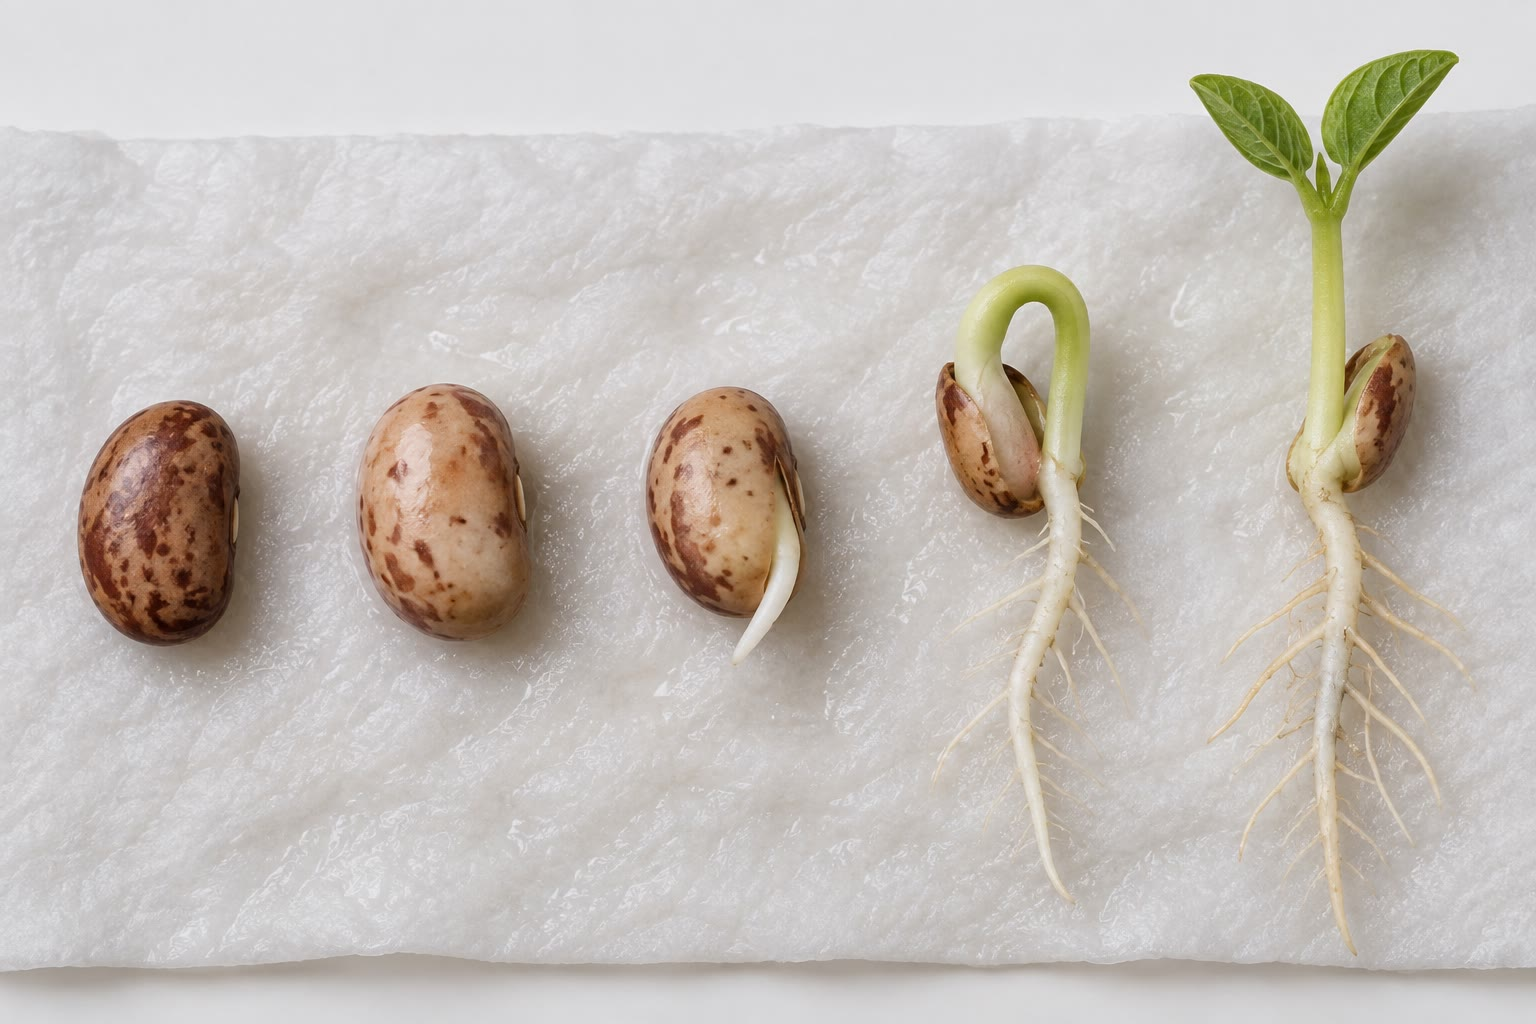
\includegraphics[width=0.66\linewidth]{images/book4/ai/b4-14-germinating-beans.jpg}

{\small A germinação do feijão: a \omterm{def:b2:angiosperm-reproduction:seed}{semente} se embebe, a radícula emerge
primeiro, o hipocótilo sobe pelo solo em forma de gancho, e o gancho se
endireita na luz quando as primeiras folhas se abrem.}
\end{omfigure}

\begin{theorem}[A germinação como aposta]\label{thm:b2:plant-flowering:bet}
\index{diversificação de riscos}
Suponha que uma fração $g$ de uma coorte de \omterm{def:b2:angiosperm-reproduction:seed}{sementes} germine a cada ano
e que o restante sobreviva no solo com probabilidade $s$ até o ano
seguinte. Num ano bom, uma \omterm{def:b2:angiosperm-reproduction:seed}{semente} que germina deixa $R_g$ \omterm{def:b2:angiosperm-reproduction:seed}{sementes};
num ano ruim, nenhuma; os anos são bons com probabilidade $p$. Uma
estratégia que germina tudo de uma vez ($g = 1$) tem, ao longo de uma
série de anos, uma taxa de crescimento de longo prazo, calculada pela
média dos $\ln$, igual a $p\ln R_g + (1 - p)\ln 0 =
-\infty$: um único ano ruim a extingue. Uma estratégia com $g < 1$
cresce nos anos bons por um fator $gR_g + (1 - g)s$ e nos anos ruins
por $(1 - g)s > 0$, de modo que sua taxa de longo prazo,
\[
r = p\ln\bigl(gR_g + (1 - g)s\bigr) + (1 - p)\ln\bigl((1 - g)s\bigr),
\]
é finita e, para $p$ não muito próximo de 1, é máxima para um $g$
intermediário. Com $R_g = 20$, $s = 0.8$ e $p = 0.7$, o ótimo fica
perto de $g = 0.7$: germinar a maior parte, guardar uma reserva. A
\omterm{def:b2:angiosperm-reproduction:seed}{dormência} não é uma falha de germinação, mas uma recusa parcial
selecionada pela evolução.
\end{theorem}
\begin{proof}
O tamanho da população após $T$ anos é o produto dos fatores anuais, de
modo que sua taxa de crescimento é a média de seus logaritmos (a taxa
média geométrica), que é o que a seleção maximiza em longas séries. Com
$g = 1$, o fator dos anos ruins é zero e o logaritmo é $-\infty$. Para
$g < 1$, os dois fatores são positivos; derivar $r$ em relação a $g$ e
igualar a derivada a zero dá o ótimo, que, para os valores citados,
fica perto de $g = 0.7$
(avaliar $r$ em $g = 0.4, 0.6, 0.8, 1$ dá $1.28$, $1.42$,
$1.40$, $-\infty$).
\end{proof}

\begin{omfigure}
\begin{tikzpicture}
\begin{axis}[
  width=0.7\linewidth, height=5.4cm,
  axis x line=bottom, axis y line=left,
  xmin=0, xmax=1, ymin=0, ymax=1.7,
  xlabel={fração que germina a cada ano, $g$}, ylabel={taxa de crescimento de longo prazo $r$},
  xlabel style={font=\small, at={(axis description cs:0.5,-0.13)}, anchor=north},
  ylabel style={font=\small},
  tick label style={font=\small}, xtick={0,0.2,0.4,0.6,0.8,1}, ytick={0,0.5,1,1.5},
  clip=false,
]
\addplot[very thick, omDef, domain=0.02:0.97, samples=100] {0.7*ln(20*x + 0.8*(1-x)) + 0.3*ln(0.8*(1-x))};
\draw[dashed, gray] (axis cs:0.7,0) -- (axis cs:0.7,1.43);
\node[font=\scriptsize, anchor=south] at (axis cs:0.7,1.45) {ótimo: guardar \qty{30}{\%} no solo};
\node[font=\scriptsize, anchor=north west, align=left] at (axis cs:0.7,0.6) {$g \to 1$: um ano ruim\\elimina a coorte};
\end{axis}
\end{tikzpicture}

{\small A \omterm{thm:b2:plant-flowering:bet}{diversificação de riscos} pela \omterm{def:b2:angiosperm-reproduction:seed}{dormência}. Com anos bons sete
vezes em dez, uma coorte que germina por inteiro acaba destruída por um
ano ruim; uma coorte que retém uma parte de suas \omterm{def:b2:angiosperm-reproduction:seed}{sementes} cresce mais
depressa a longo prazo.}
\end{omfigure}

\section{Exercícios}

\begin{exercise}[$\star$]\label{exo:b2:plant-flowering:1}
Distinga os \omterm{def:b2:plant-meristems:meristem}{meristemas} vegetativos, de inflorescência e florais, e diga
quais são determinados.
\end{exercise}

\begin{exercise}[$\star$]\label{exo:b2:plant-flowering:2}
Defina \omterm{prop:b2:plant-flowering:photoperiod}{plantas de dia curto}, de dia longo e neutras, com um exemplo de
cada, e diga o que uma \omterm{prop:b2:plant-flowering:photoperiod}{planta de dia curto} mede de fato.
\end{exercise}

\begin{exercise}[$\star$]\label{exo:b2:plant-flowering:3}
Dê a identidade de órgão de cada verticilo no tipo selvagem e nos três
mutantes simples do \omterm{prop:b2:plant-flowering:abc}{modelo ABC}.
\end{exercise}

\begin{exercise}[$\star$]\label{exo:b2:plant-flowering:4}
Cite quatro sinais que quebram a \omterm{def:b2:angiosperm-reproduction:seed}{dormência} das \omterm{def:b2:angiosperm-reproduction:seed}{sementes} e, para cada
um, a estação ou o lugar que ele indica.
\end{exercise}

\begin{exercise}[$\star\star$]\label{exo:b2:plant-flowering:5}
Uma \omterm{prop:b2:plant-flowering:photoperiod}{planta de dia curto} tem uma noite crítica de \qty{10}{h}. Diga se
ela floresce sob: \qty{16}{h} de luz/\qty{8}{h} de escuro;
\qty{12}{h}/\qty{12}{h}; \qty{12}{h} de luz, \qty{6}{h} de escuro, um
minuto de luz, \qty{6}{h} de escuro; \qty{8}{h} de luz, \qty{4}{h} de
escuro, \qty{4}{h} de luz, \qty{8}{h} de escuro.
\end{exercise}

\begin{exercise}[$\star\star$]\label{exo:b2:plant-flowering:6}
Uma folha de uma \omterm{prop:b2:plant-flowering:photoperiod}{planta de dia curto} induzida é enxertada numa \omterm{prop:b2:plant-flowering:photoperiod}{planta de
dia longo} mantida em dias longos, e a \omterm{prop:b2:plant-flowering:photoperiod}{planta de dia longo} floresce. O
que isso mostra sobre o \omterm{def:b2:plant-flowering:florigen}{florígeno}? E se o enxerto for feito com uma
folha induzida, mas com o floema interrompido no pecíolo?
\end{exercise}

\begin{exercise}[$\star\star$]\label{exo:b2:plant-flowering:7}
O frio silencia o repressor a $\alpha = 0.05$ por dia, e a floração
exige $f < 0.15$. Quantos dias frios são necessários? Um inverno tem
três períodos frios de 15, 12 e 20 dias, separados por degelos: a
planta está vernalizada? E se $\alpha$ fosse $0.02$?
\end{exercise}

\begin{exercise}[$\star\star$]\label{exo:b2:plant-flowering:8}
Explique, em termos de cromatina, por que a memória de uma planta
vernalizada se perde em suas \omterm{def:b2:angiosperm-reproduction:seed}{sementes}, e por que isso é útil.
\end{exercise}

\begin{exercise}[$\star\star$]\label{exo:b2:plant-flowering:9}
\omterm{def:b2:angiosperm-reproduction:seed}{Sementes} de alface recebem, no escuro, as sequências: V; V depois VE;
V, VE, V; V, VE, V, VE (V: vermelho; VE: vermelho extremo). Preveja a
germinação em cada caso e explique em termos das duas formas do
fitocromo.
\end{exercise}

\begin{exercise}[$\star\star\star$]\label{exo:b2:plant-flowering:10}
No modelo de \omterm{thm:b2:plant-flowering:bet}{diversificação de riscos} com $R_g = 20$, $s = 0.8$, calcule
a taxa de crescimento de longo prazo para $g = 0.4$, $0.6$, $0.8$ e $1$
quando $p = 0.7$, e de novo quando $p = 0.95$. Como o ótimo se desloca,
e o que isso prevê para os desertos em comparação com os prados?
\end{exercise}

\begin{exercise}[$\star\star\star$]\label{exo:b2:plant-flowering:11}
Preveja a \omterm{def:b2:angiosperm-reproduction:flower}{flor} produzida pela expressão de um gene da classe B nos
quatro verticilos; pela expressão da classe C nos quatro; por um duplo
mutante sem A e B. Depois, explique por que a \omterm{def:b2:angiosperm-reproduction:flower}{flor} sem C continua
formando verticilos.
\end{exercise}

\begin{exercise}[$\star\star\star$]\label{exo:b2:plant-flowering:12}
``Uma planta decide florescer integrando sinais que não pode
controlar.'' Discuta as três integrações deste capítulo --- do
comprimento do dia, do frio, dos anos no banco de \omterm{def:b2:angiosperm-reproduction:seed}{sementes} --- e contra
o que um integrador protege a planta, que um simples limiar não
protegeria.
\end{exercise}

\section{Problema: O calendário do produtor}

\begin{problem}[{Problema de fim de semana --- um produtor de
crisântemos programa a floração com luzes, um melhorista de trigo conta
o frio, a flor dobrada de um florista é explicada e a dormência de um
lote de sementes é modelada, até o comprimento de noite que desencadeia
a floração da cultura, os dias frios de que o trigo precisa e a melhor
fração de germinação}]
\label{pb:b2:plant-flowering:1}
O crisântemo é uma \omterm{prop:b2:plant-flowering:photoperiod}{planta de dia curto} com uma noite crítica de
\qty{9.5}{h}; a indução exige \num{12} noites indutivas consecutivas, e
as \omterm{def:b2:angiosperm-reproduction:flower}{flores} se abrem \num{8} semanas após a indução. Em novembro, a
estufa fica no escuro das 17:00 às 07:30. O trigo de inverno tem
$\alpha = 0.06$ por dia frio e floresce quando $f < 0.10$. Lote de
\omterm{def:b2:angiosperm-reproduction:seed}{sementes}: $R_g = 15$, $s = 0.7$, anos bons com probabilidade $p$.

\medskip
\noindent\textbf{Parte I --- A estufa.}
\begin{enumerate}
  \item Em junho, a noite natural dura \qty{8}{h}. A cultura vai
        florescer? O que o produtor precisa fazer para vender \omterm{def:b2:angiosperm-reproduction:flower}{flores} em
        agosto?
  \item O produtor cobre a cultura com um pano preto das 19:00 às
        07:00. Que comprimento de noite a planta percebe, e quando a
        cobertura precisa começar para uma abertura em 15~de agosto?
  \item Em novembro, a noite natural dura \qty{14}{h} e o produtor quer
        \emph{adiar} a floração para o Natal. Proponha um esquema de
        iluminação e explique por que um breve lampejo basta.
  \item O lampejo é dado às 21:00, e não às 00:00, e a indução não é
        impedida. Explique com o comprimento crítico da noite.
  \item Numa das doze noites, o pano não é colocado. Preveja, e diga o
        que um carrapicho teria feito.
  \item O lampejo é dado com luz verde e falha; com luz vermelha,
        funciona; vermelho seguido de vermelho extremo falha. Explique.
  \item Uma única folha de uma planta induzida é enxertada numa planta
        mantida em dias longos. Preveja, e diga o que isso identifica.
\end{enumerate}

\medskip
\noindent\textbf{Parte II --- O trigo.}
\begin{enumerate}[resume]
  \item De quantos dias frios o trigo precisa?
  \item Semeado em outubro, ele recebe 10 dias frios em novembro, um
        dezembro ameno, 25 em janeiro e 12 em fevereiro. Quando ele fica
        vernalizado?
  \item Semeado em março, ele recebe 6 dias frios. Ele floresce nesse
        verão? Qual é a consequência agrícola?
  \item Um mutante não tem o repressor. Preveja seu comportamento e
        diga por que os melhoristas chamam esses trigos de ``trigos de
        primavera''.
  \item Explique por que a memória do frio sobrevive às divisões do
        \omterm{def:b2:plant-meristems:meristem}{meristema} durante a primavera, mas não à \omterm{def:b2:meiosis-heredity:meiosis}{meiose} que forma a
        geração seguinte.
  \item Por que o frio precisa ser contado no \omterm{def:b2:plant-meristems:meristem}{meristema}, e não nas
        folhas, ao contrário do comprimento do dia?
\end{enumerate}

\medskip
\noindent\textbf{Parte III --- O florista.}
\begin{enumerate}[resume]
  \item Uma rosa dobrada tem pétalas onde deveriam estar os \omterm{def:b2:angiosperm-reproduction:flower}{estames} e
        algumas pétalas extras no centro. Que classe de gene falhou? Dê
        a fórmula dos verticilos.
  \item Essas rosas são estéreis como genitores masculinos, mas às vezes
        formam \omterm{def:b2:angiosperm-reproduction:seed}{sementes}. Explique os dois fatos a partir do \omterm{prop:b2:plant-flowering:abc}{modelo ABC}.
  \item Uma boca-de-leão tem \omterm{def:b2:angiosperm-reproduction:flower}{estames} no lugar das pétalas e \omterm{def:b2:angiosperm-reproduction:flower}{carpelos} no
        lugar das sépalas. Que classe falhou?
  \item Preveja a \omterm{def:b2:angiosperm-reproduction:flower}{flor} de uma planta em que a classe C é expressa no
        verticilo 1, além de seus verticilos normais.
  \item Por que as mesmas \omterm{def:b2:genome-diversification:mutation}{mutações} produziram as mesmas transformações
        numa rosa, numa boca-de-leão e em \emph{Arabidopsis}, plantas
        separadas por cem milhões de anos?
  \item No verticilo 2 de uma \omterm{def:b2:angiosperm-reproduction:flower}{flor} selvagem, A e B estão ativas. Preveja
        o órgão se apenas B estivesse ativa ali.
\end{enumerate}

\medskip
\noindent\textbf{Parte IV --- O lote de \omterm{def:b2:angiosperm-reproduction:seed}{sementes}.}
\begin{enumerate}[resume]
  \item Calcule a taxa de crescimento de longo prazo $r$ para $g = 0.5$,
        $0.7$ e $0.9$ quando $p = 0.8$.
  \item Qual dos três é o melhor? O que acontece com $g = 1$?
  \item Recalcule para $p = 0.5$ (um deserto). Qual $g$ é o melhor
        agora?
  \item Um produtor semeia o lote inteiro numa só lavoura num ano bom e
        colhe $R_g$ por \omterm{def:b2:angiosperm-reproduction:seed}{semente}. Explique por que sua estratégia difere
        da estratégia da planta e o que ele precisa fazer para conservar
        a variedade durante um ano ruim.
  \item As \omterm{def:b2:angiosperm-reproduction:seed}{sementes} exigem luz para germinar. Explique o sentido
        adaptativo disso para uma \omterm{def:b2:angiosperm-reproduction:seed}{semente} pequena, e preveja o que a
        aração faz com o banco de \omterm{def:b2:angiosperm-reproduction:seed}{sementes}.
  \item Enuncie o resultado: o comprimento crítico da noite e o esquema
        de cobertura, a necessidade de frio do trigo e o melhor $g$ para
        $p = 0.8$ e $p = 0.5$.
\end{enumerate}
\end{problem}
